\chapter{Technology Review}
This chapter discusses the different technologies used in throughout the
project. It discusses the the advantages and disadvantages of each technology 
and why certain technologies were used over others.

\section{Overview}
This project is comprised of React as the frontend, Flask as the server which is
hosted on PythonAnywhere, MongoDB as the database for user authentication, Firebase as the database to store sorts, and Docker and Firebase to deploy/host the application. Throughout the project, the following technologies were also used 
and tested before the above was ultimately chosen:
\begin{itemize}
    \item Angular/Ionic
    \item Django
    \item MySQL
    \item Amazon Web Services
    \item Heroku
\end{itemize}

\newpage
\section{Main Technologies}
This section will discuss the main technologies currently in use in the web 
application. The preceding section will discuss other technologies tried but 
ultimately weren't incorporated. 

\subsection{React}
\par
\medskip
\begin{center}
    
\includegraphics[width=8cm,height=3.3cm,keepaspectratio]{images/react}
\end{center}
React (also known as React.js or ReactJS) is a JavaScript library for building 
user interfaces \cite{react_wiki}. It is maintained by Facebook and a community of individual 
developers and companies \cite{react_docs}.
\par
\bigskip
React can be used as a base in the development of single-page or mobile 
applications. However React is only concerned with rendering data to the DOM and
so creating React applications usually requires the use of additional libraries 
for state management and routing. Redux and React Router are respective examples
of such libraries. 

\subsubsection{Advantages}
React has many advantages, several of which apply to this project:

\begin{itemize}
    \item \textbf{Wide React and Redux toolset} - Both React and Redux come with a set of related tools that make a developer’s life easier. For instance, React Developer Tools extension for Chrome and a similar one for Firefox allow for examining component hierarchies in the virtual DOM and editing states and properties. Additionally, you can check React Sight that visualizes state and prop trees; Reselect DevTools that helps with debugging and visualizing Reselect, a selector library for Redux. Redux DevTools Profiler Monitor allows for profiling actions in well.
    \item \textbf{Faster Rendering} - Building a high-load application is essential to consider how the structure will impact the overall app performance. Even latest platforms and engines can't ensure the absence of bottlenecks, because DOM (Document Object Model) is tree-structured and even small changes at the upper layer can cause awful ripples to the interface. To solve the issue, Facebook development team has introduced Virtual DOM – currently, one of the benefits of using React for heavy loaded and dynamic software solutions. As the name suggests, it is a virtual representation of the document object model, so all the changes are applied to the virtual DOM first and then, using diff algorithm, the minimal scope of necessary DOM operations is calculated. Finally, the real DOM tree is updated accordingly, ensuring minimum time consumed. This method guarantees better user experience and higher app performance.
    \item \textbf{Guaranteed Stable Code} - To make sure that even small changes that take place in the child structures won't affect their parents, ReactJS uses only downward data flow. Changing an object, developers just modify its state, make changes, and, after that, only particular components will be updated. This structure of data binding ensures code stability and continuous app performance.
\end{itemize}

\subsubsection{Disadvantages}
There are a few disadvantages to using React:

\begin{itemize}
    \item \textbf{Poor Documentation} - The problem with documentation traces back to constant releases of new tools. Different and new libraries like Redux and Reflux are promising to accelerate the work of a library or improve the entire React ecosystem. At the end, developers struggle with integrating these tools with ReactJS. Some members of the community think that React technologies are updating and accelerating so fast that there is no time to write proper instruction. To solve this, developers write their own documentation for specific tools used by them in current projects.
    \item \textbf{JSX as a barrier} - ReactJS uses JSX. It’s a syntax extension, which allows mixing HTML with JavaScript. JSX has its own benefits (for instance, protecting code from injections), but some members of the development community consider JSX to be a serious disadvantage. Developers and designers complain about JSX’s complexity and consequent steep learning curve.
    \item \textbf{Limitations in certain aspects} - As discovered with this project, certain tasks that can be done easily in other languages can't be done as easily in React. For example, if you wish to list all files in Firebase Storage using HTML, this can be done easily using a standard table to list the files. However, in React, this does not seem to be possible at the moment as it only seems to be possible to list one file at a time. Fortunately, the React community has developed libraries to get around these problems.
\end{itemize}

\newpage
\subsubsection{Purpose in application}
A vast majority of the application was written in React, namely the visualization aspect \cite{sorting_howto}, user registration and login forms, recording of sorts \cite{screenflow}, upload of sorts, and viewing of sorts. Below discusses how each of the main parts of main page were developed:
\par
\bigskip
\paragraph{Main Page}
\begin{center}
    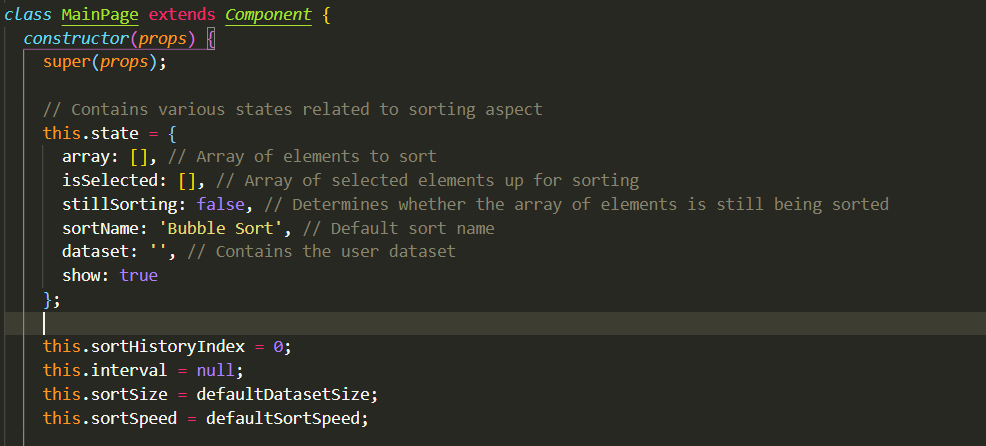
\includegraphics[width=12cm,height=12cm,keepaspectratio]{images/mainpage1}
\end{center}
In the React sense, “state” is an object that represents the parts of the app that can change. Each component can maintain its own state, which lives in an object called this.state. If you’d like your app to do anything – if you want interactivity, adding and deleting things, logging in and out – that will involve state. In the context of this application, state contains information on the array of elements to be sorted, whether or not a certain element has been selected for sorting, if the application is still sorting the array, the current sort selected and the user's data set. The application will change and update these values as necessary.
\newpage
\begin{center}
    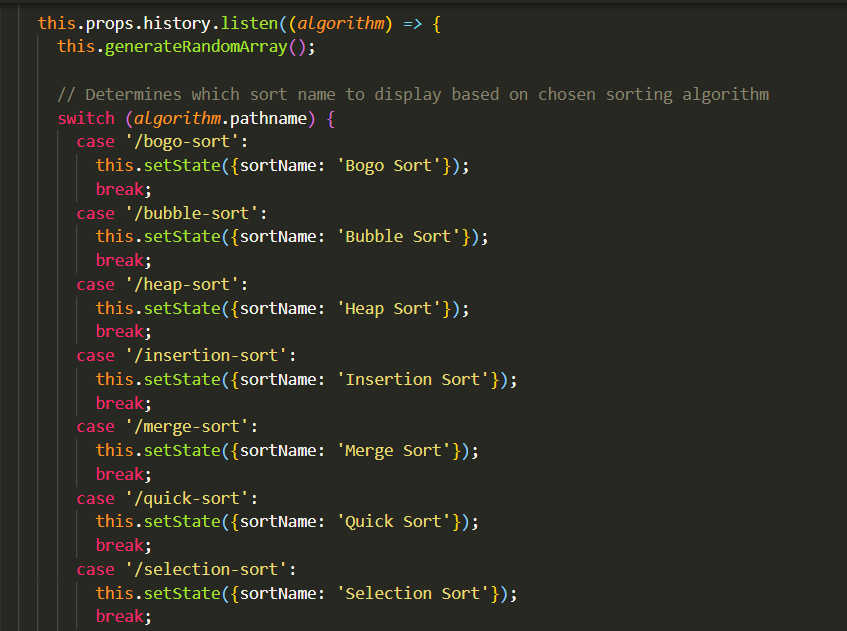
\includegraphics[width=12cm,height=12cm,keepaspectratio]{images/mainpage2}
\end{center}
Here, the application simply sets the current name of the selected sort and displays it the user.

\begin{center}
    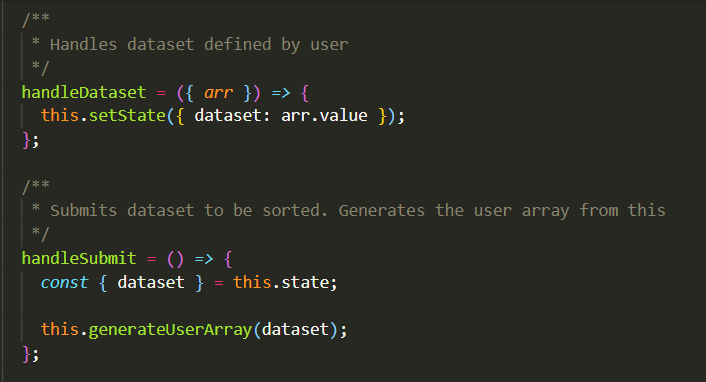
\includegraphics[width=15cm,height=6cm,keepaspectratio]{images/mainpage3}
\end{center}
Here the application handles the user's data set: handleDataset() will first save the user's data set to an array in state. handleSubmit() will submit the data set to be sorted i.e. the application will generate a visual representation of the user's data set. The user can then choose what sorting algorithm to apply and visualize.

\begin{center}
    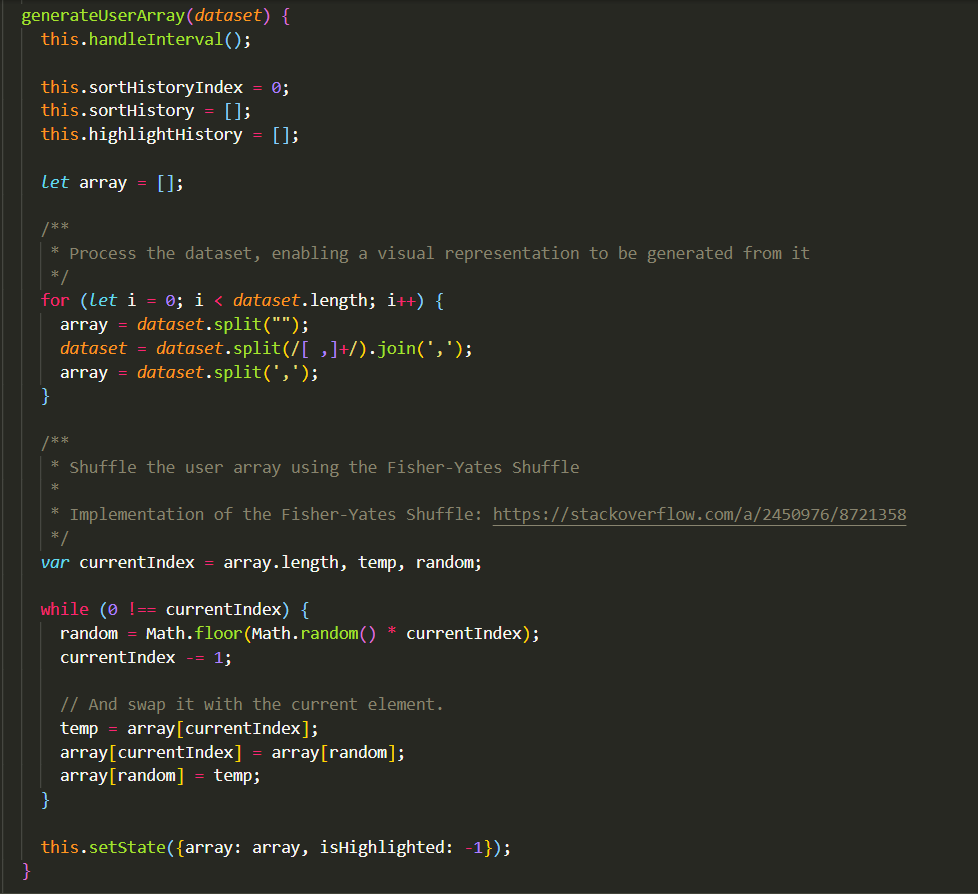
\includegraphics[width=10cm,height=10cm,keepaspectratio]{images/mainpage4}
\end{center}
To generate a visual representation of the array, I first needed to process the user's input correctly. The data set was iterated over and any unnecessary character was removed. The contents of the data set was then stored in array. Next, I needed to ensure the array was always shuffled when a visual representation of it was generated. To do this, I used the Fisher-Yates shuffle which is an algorithm for generating a random permutation of a finite sequence—in plain terms, the algorithm shuffles the sequence. The algorithm effectively puts all the elements into a hat - it continually determines the next element by randomly drawing an element from the hat until no elements remain.
\par
\bigskip
\begin{center}
    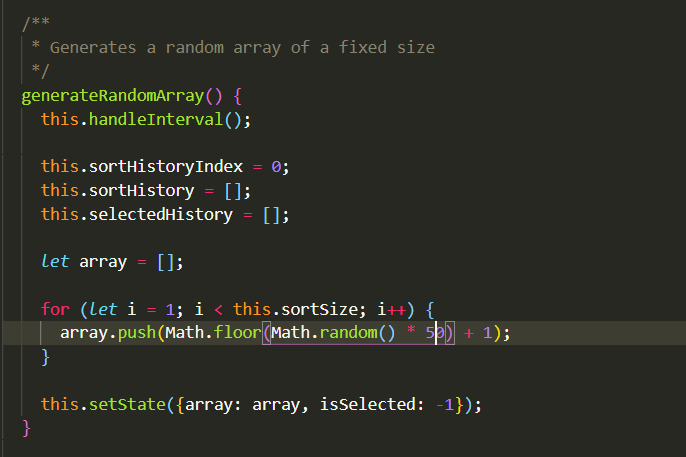
\includegraphics[width=10cm,height=10cm,keepaspectratio]{images/mainpage5}
\end{center}
To generate a random array, a sort size was first set. A random array of elements was then generated of that size.

\begin{center}
    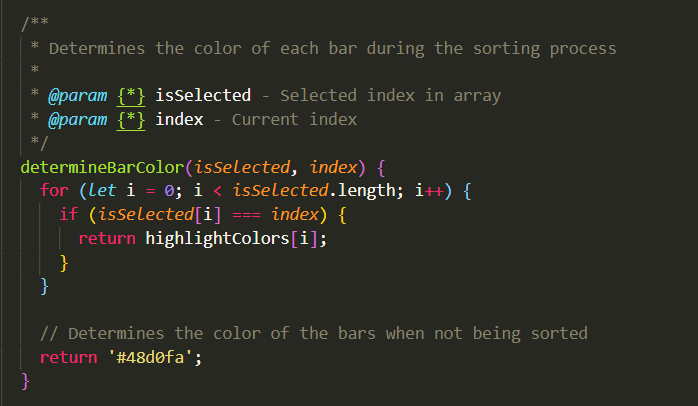
\includegraphics[width=10cm,height=9cm,keepaspectratio]{images/mainpage7}
\end{center}
setColor() determines the color of bars that represent each element in the array. In this function, the application iterates over the array of selected elements, and if index i of that array is the index, the bar will be changed to the color in index i of highlightedColors.

\newpage
\begin{center}
    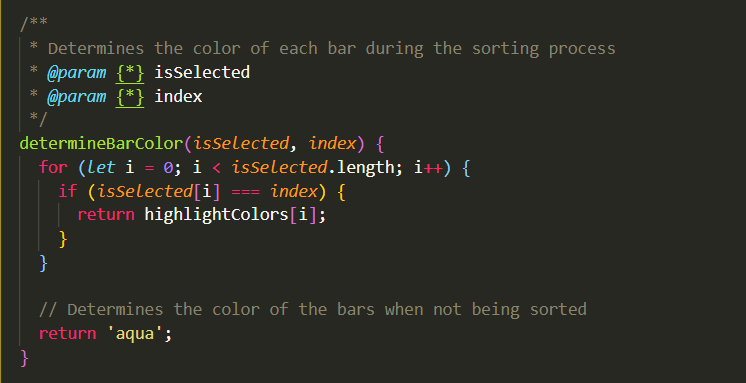
\includegraphics[width=10cm,height=9cm,keepaspectratio]{images/mainpage6}
\end{center}
This piece of code will execute the correct sorting algorithm. The application will first get 'path', which is comprised of location.pathname. Then, based on this, will pass the array, sortHistory, and selectedHistory to the correct algorithm. Each of these algorithms are discussed in section 4.2.1 of the System Design chapter. The visualization of the array being sorted will then be shown.

\begin{center}
    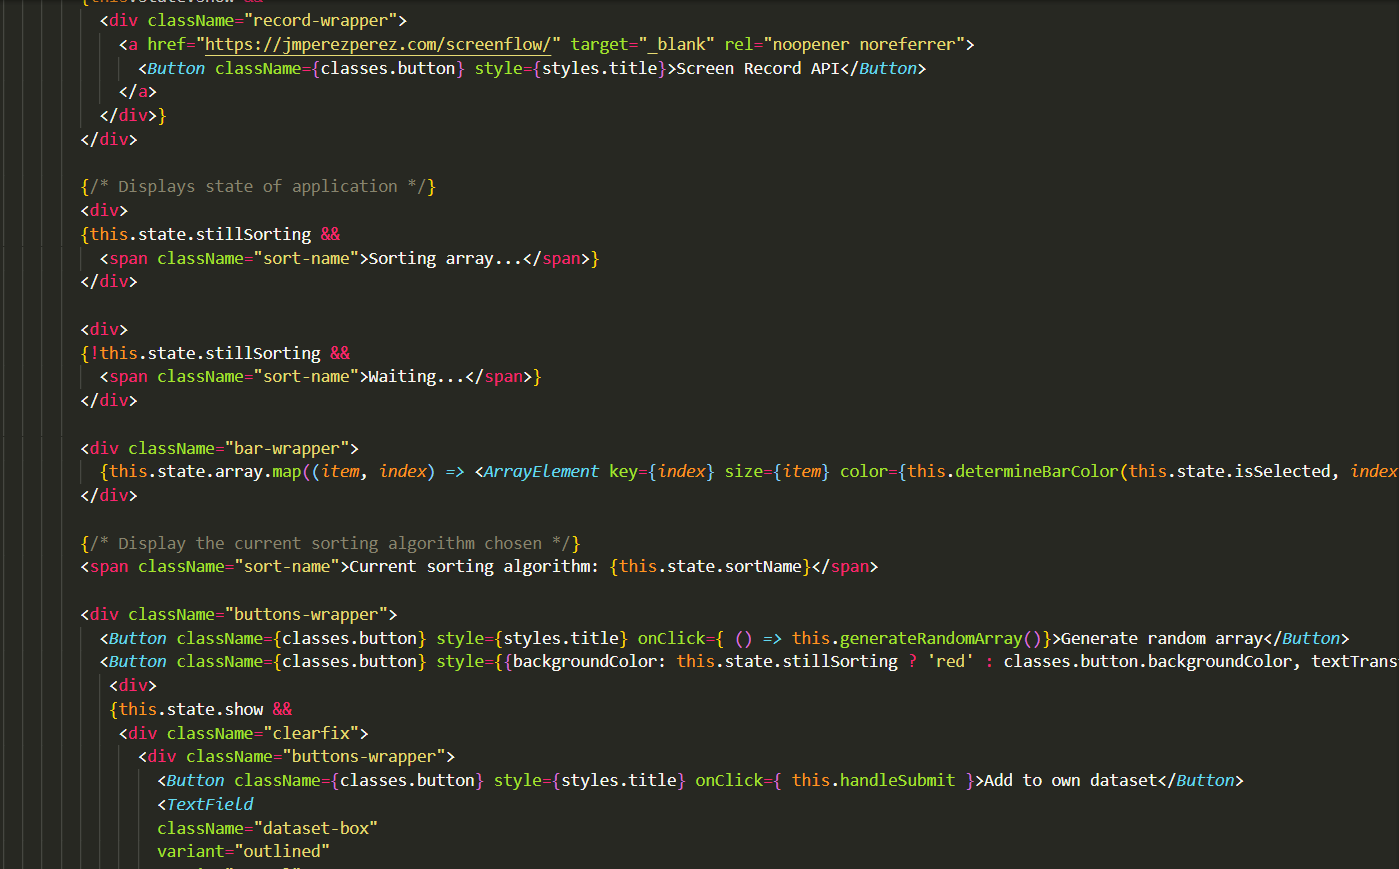
\includegraphics[width=10cm,height=9cm,keepaspectratio]{images/mainpage8}
\end{center}
The render() function renders all the appropriate GUI, ranging from the toolbar for the various sorting algorithm, the bars themselves, and the various buttons for interacting with the application.

\paragraph{MainToolbar}
\begin{center}
    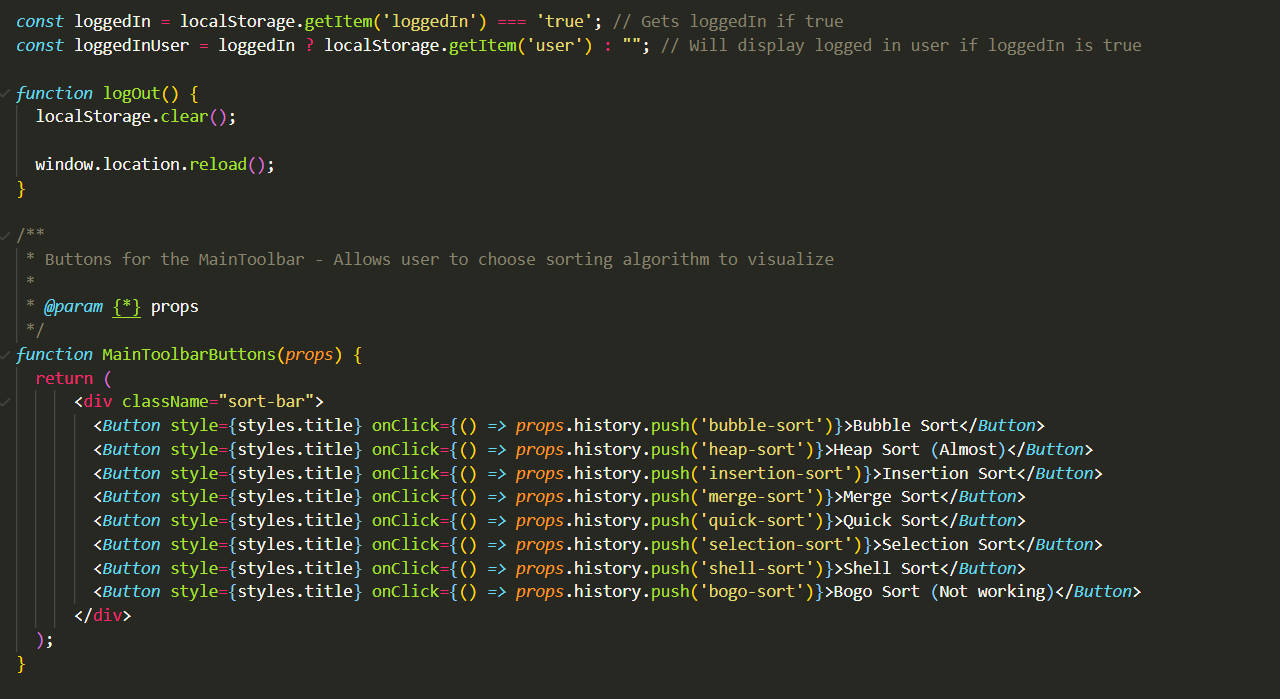
\includegraphics[width=10cm,height=10cm,keepaspectratio]{images/toolbar1}
\end{center}
When a component is rendered by React Router, that component is passed three different props: location, match, and history. This history prop comes from the History library and has properties on it related to routing. In this case, the one we’re interested in is history.push. What it does is it pushes a new entry into the history stack - redirecting the user to another route. When an algorithm is selected, the correct route to the algorithm is selected. This allows the algorithm to be correctly visualized.

\begin{center}
    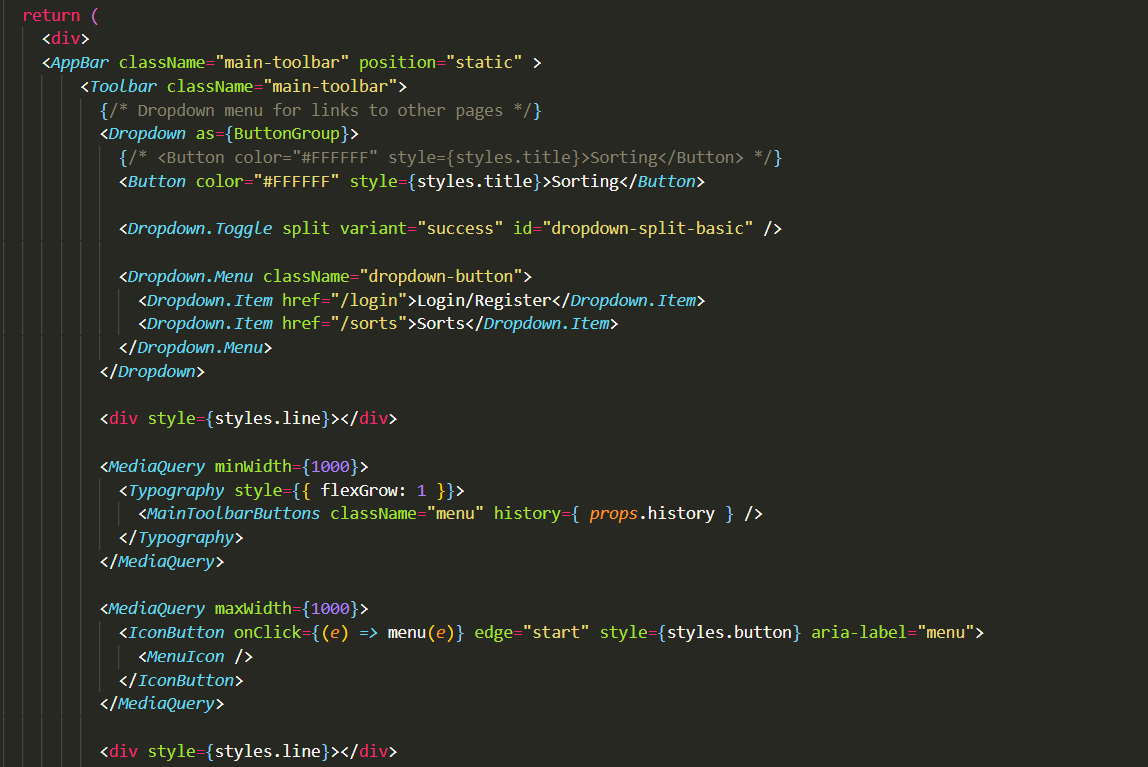
\includegraphics[width=10cm,height=10cm,keepaspectratio]{images/toolbar2}
\end{center}
The above code simply renders the toolbar. The toolbar is 'exported' as a component, which can then be used in other React pages.

\newpage
\paragraph{User Functions}
\begin{center}
    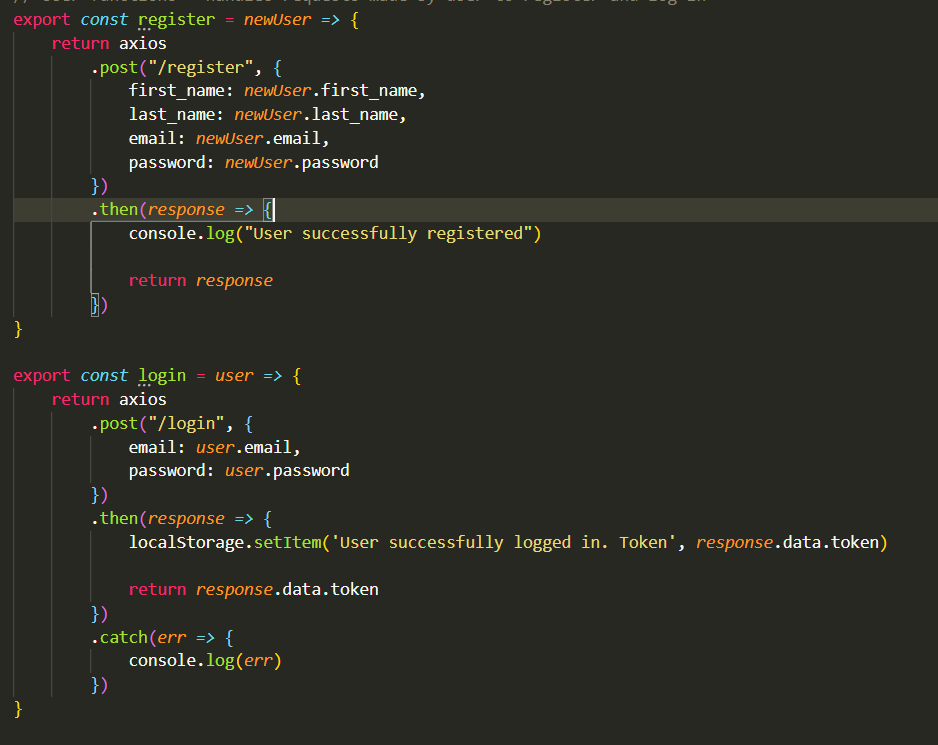
\includegraphics[width=8cm,height=10cm,keepaspectratio]{images/userfuncs}
\end{center}
The user functions file handles the register and login requests \cite{frm_logreg}. These requests are delegated to the Flask server, where the appropriate action is taken. A response will then be returned based on the initial request.

\bigskip
\paragraph{Login Page}
\begin{center}
    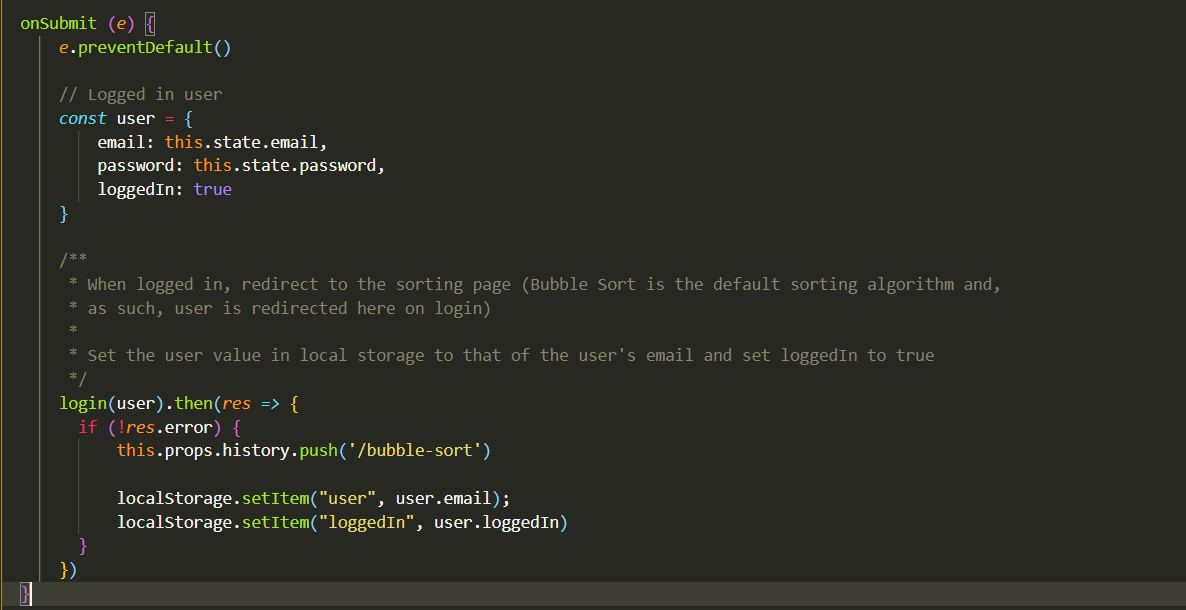
\includegraphics[width=6cm,height=10cm,keepaspectratio]{images/login2}
    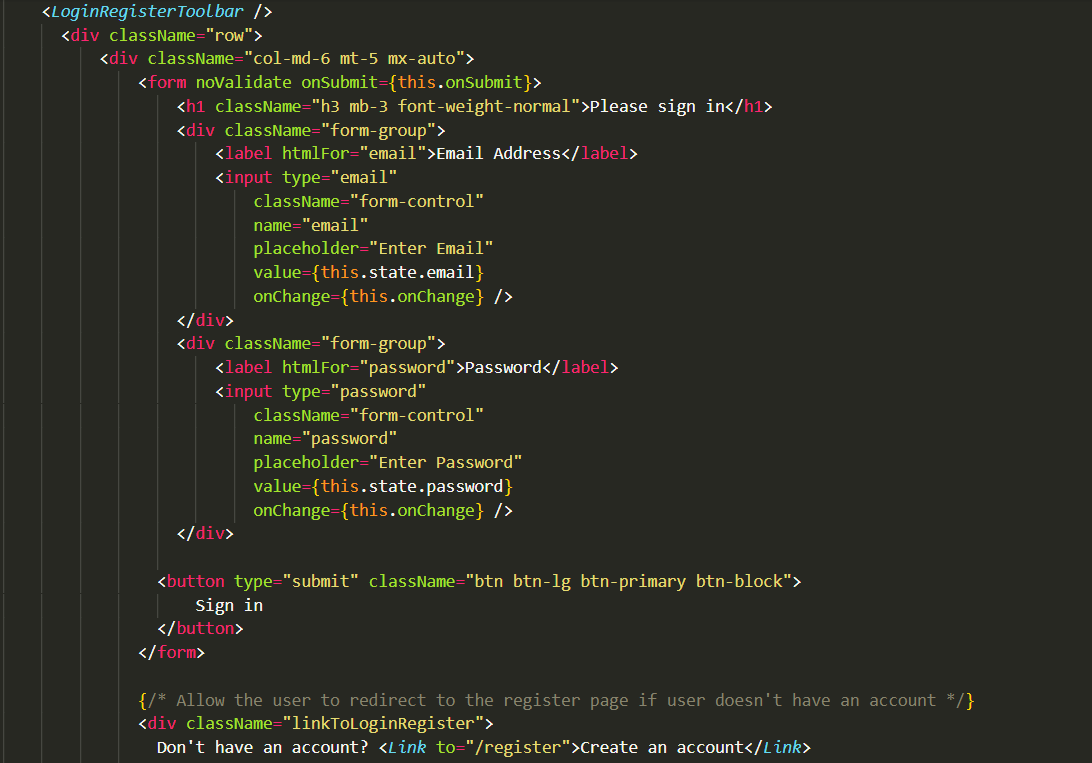
\includegraphics[width=6cm,height=10cm,keepaspectratio]{images/login1}
\end{center}
The Login page uses the login function defined in the user functions file to handle a login request. If the user has successfully logged in, the local storage will be appropriately updated and the application will redirect to the sorting page. The login form is a simple HTML inspired form.

\newpage
\paragraph{Register Page}
\begin{center}
    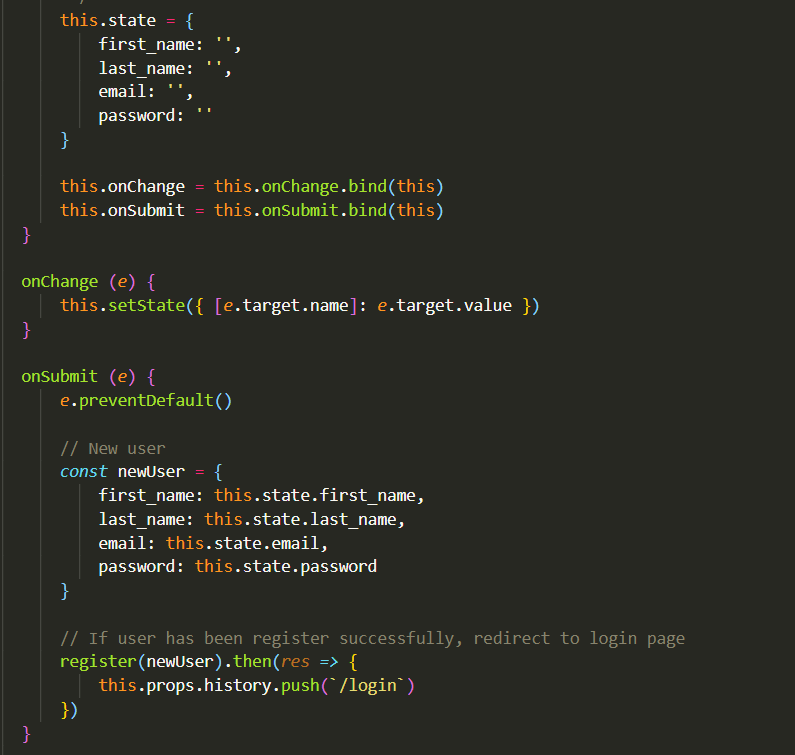
\includegraphics[width=8cm,height=10cm,keepaspectratio]{images/register1}
\end{center}
The Register page, like the Login page, uses the register function defined in the user functions file to handle a register request. If the user has successfully registered an account, the application will redirect to the login page where the user can then log in to their newly created account. The register form is a simple HTML inspired form.

\newpage
\subsection{Flask}
\par
\medskip
\begin{center}
    
\includegraphics[width=8cm,height=3.3cm,keepaspectratio]{images/flask}
\end{center}
Flask is a micro web framework written in Python \cite{flask_docs}, \cite{python_docs}. It is classified as a 
micro-framework because it does not require particular tools or libraries. It 
has no database abstraction layer, form validation, or any other components 
where pre-existing third-party libraries provide common functions. However, 
Flask supports extensions that can add application features as if they were 
implemented in Flask itself. Some of the main features of Flask are:

\begin{itemize}
    \item Development server and debugger
    \item Integrated support for unit testing
    \item Support for secure cookies (client side sessions)
    \item 100\% WSGI 1.0 compliant
\end{itemize}

For this project, Flask was used as the middle-man for the React application and
MongoDB database. Certain functionality, such as enabling users to register, 
login, upload sorts, etc. are written in Flask which are then accessed by the 
React application when needed. The Flask application is hosted on 
PythonAnywhere.

\subsubsection{Advantages}
There are a number of advantages to using Flask:

\begin{itemize}
    \item \textbf{Flexibility} - There are very few parts of Flask that cannot
    be easily and safely altered, due to its simplicity and minimality.
    \item \textbf{Modularity} - Modular code provides a huge number of benefits.
    With Flask, you have the ability to create multiple Flask applications or 
    servers, distributed across a large network of servers, each with specific 
    purposes. This creates more efficiency, better testability, and better 
    performance.
    \item \textbf{Performance} - A micro framework can be thought of as being 
    slightly more “low-level” than something like Django. There are fewer levels
    of abstraction between the user and the database, the requests, the cache, 
    etc. so performance is inherently better from the start.
    \item \textbf{Scalable} - Flask can be argued to be more scalable than 
    monoliths if using modern methods. Today, applications are often running in 
    containers or using cloud computing with auto-scaling. Applications do not 
    typically “scale” themselves. The infrastructure scales. With a smaller 
    application, it's easier to deploy instances across thousands of server 
    easily to handle increased traffic/load. For example, it's partly the reason
    why Pinterest needed to migrate from Django to Flask as they grew to support
    more of a micro-services pattern.
    \item \textbf{Simpler Development} - If one understands Python well, then 
    you’ll be able to move around and contribute to a Flask application easily. 
    It’s less opinionated so there are fewer standards to learn.
\end{itemize}

\subsubsection{Disadvantages}
There are a few disadvantages to using Flask:

\begin{itemize}
    \item \textbf{Community} - The monoliths provide such a large toolset,
    focused on providing solutions for a larger set of use cases out of the box,
    that they typically have a larger community. This means more eyes on the
    code, more code reviews, and better-tested core code. This is a little bit
    of a generalization though.
    \item \textbf{Fewer tools} -  You don’t have a full toolset underneath you.
    So you may need to build more on your own or search out extensions/libraries
    from the community.
    \item \textbf{Not standardized} - While Flask is simple, it’s
    not very opinionated. A Python developer without Flask experience will get 
    adjusted to a Flask application quicker than a Python developer without 
    Django experience would get adjusted to a Django application. But Django is 
    building up a large group of talent who knows the framework very well. A 
    Python developer with Django experience will get adjusted to a new Django 
    app quicker than a Python developer with Flask experience would get adjusted
    to a large Flask application.
\end{itemize}

\newpage
\subsubsection{Purpose in application}
The backend aspect of the application was written in Python/Flask \cite{frm_logreg}. The serve.py script handles requests made by the user, such as attempting to register for an account and attempting to login. Below discusses how this is achieved:

\begin{center}
    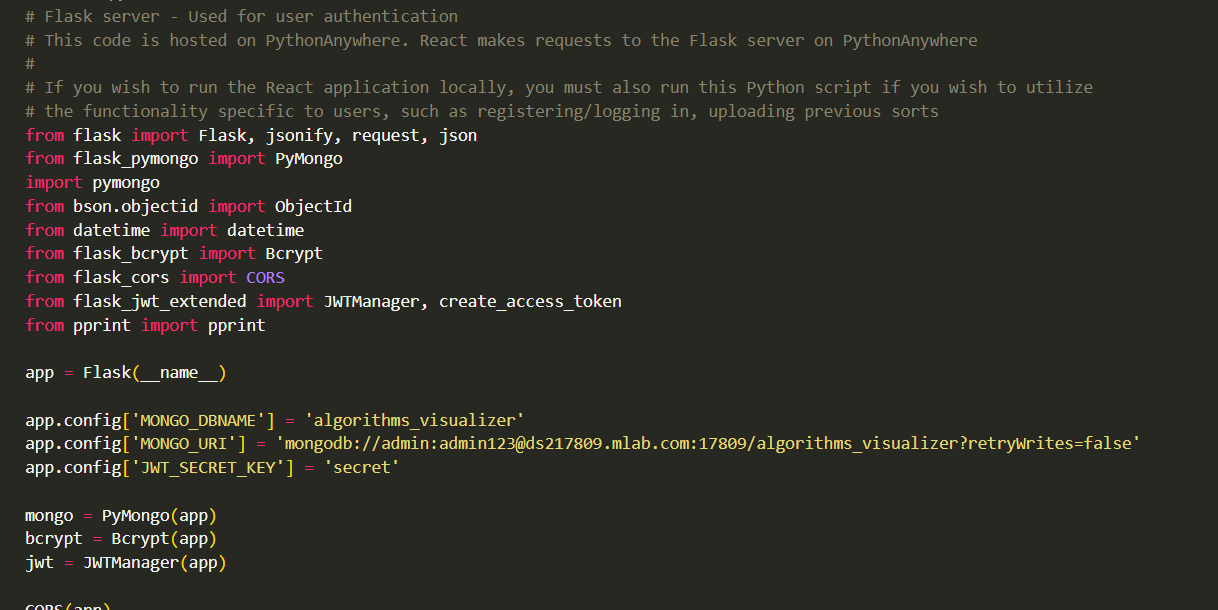
\includegraphics[width=13cm,height=13cm,keepaspectratio]{images/backend1}
\end{center}
The user authentication aspect uses a lot of different libraries to achieve the end result. The most notable libraries used and how they fit into this script are as follows:

\begin{itemize}
    \item Flask-PyMongo - MongoDB was chosen as one of the databases used in this application. MongoDB is an open source database that stores flexible JSON-like “documents,” which can have any number, name, or hierarchy of fields within, instead of rows of data as in a relational database. MongoDB as a persistent, searchable repository of Python dictionaries - this is how PyMongo actually represents MongoDB documents.
    \item Flask-Bcrypt - Flask-Bcrypt is a Flask extension that provides bcrypt hashing utilities.
    \item Flask-CORS - A Flask extension for handling Cross Origin Resource Sharing (CORS).
    \item Flask-JWT-Encoded - An open source Flask extension that provides JWT support. Adds support for using JSON Web Tokens (JWT) to Flask for protecting views. 
\end{itemize}

\newpage
To connect to the Mongo database, the database name, it's URI, and the secret key are defined. PyMongo will then connect to the MongoDB database. The Flask app object is also passed to Bcrypt, and the Flask-JWT extension is setup \cite{mlab_docs}.

\begin{center}
    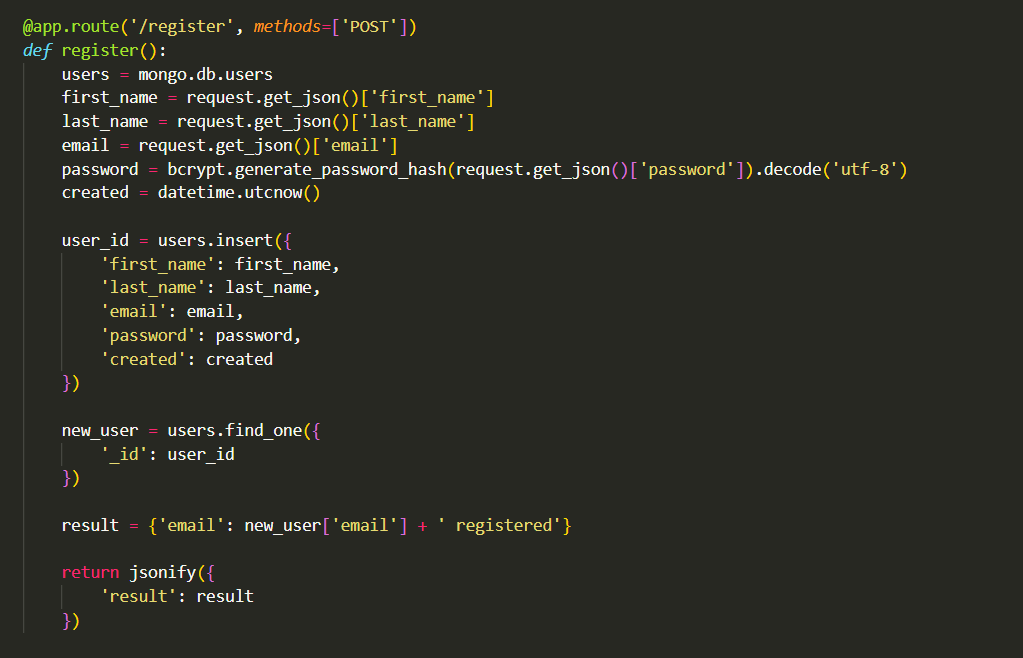
\includegraphics[width=13cm,height=13cm,keepaspectratio]{images/backend2}
\end{center}
The register method allows a user to create an account. Firstly, the script gets a handle on the database itself using \lstinline{users = mongo.db.users}. Four values are passed to the database: the user's first name, the user's last name, the user's email, and the user's password. 

\medskip
\lstinline{first_name = request.get_json()['first_name']}
\newline
\lstinline{last_name = request.get_json()['last_name']}
\newline
\lstinline{email = request.get_json()['email']}
\newline
\lstinline{password = bcrypt.generate_password_hash(request.get_json()['password']).decode('utf-8')}

\bigskip
In the case of the user's password, Bcrypt is used to generate a password hash of the user's password before being passed to the database. When inserting a user into the database, the time and date the user's account was created is also passed to the database.

\bigskip
\lstinline{user_id = users.insert(...} will then create a new document (user) in the MongoDB database with these details. 

\newpage
\begin{center}
    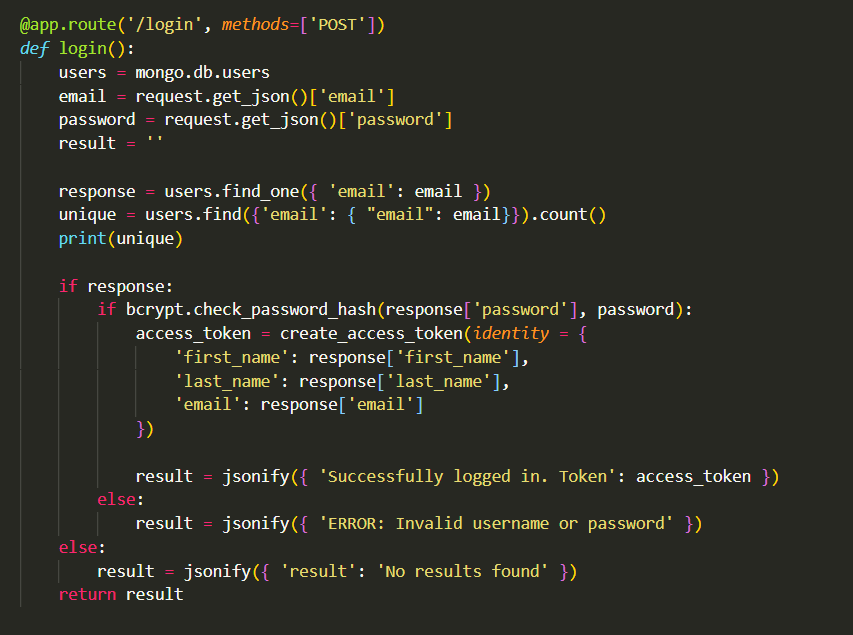
\includegraphics[width=13cm,height=13cm,keepaspectratio]{images/backend3}
\end{center}
The login method allows a user to a login into their account. To log in, the user needs to provide two details: their email and their password. The script will search the database by user's emails. If the script finds the provided email and the hash of the provided password is equal to that of the hashed password linked to the account the user is attempting to log into, the script will create an access token and the user will be logged into the application. 

\bigskip
Again, the script gets a handle on the database itself using \lstinline{users = mongo.db.users}. Using \lstinline{response = users.find_one({ 'email': email })}, the script will try and find a matching email with the one provided. 

\bigskip
\lstinline{if response:}
\newline
\quad\lstinline{if bcrypt.check_password_hash(response['password'], password):}

\bigskip
This will check if \lstinline{response} returns true and if the hash of the password associated with the account found is correct. If so, the access token will created and the user will be logged in.

\newpage
\subsection{PythonAnywhere}
\par
\medskip
\begin{center}
    
\includegraphics[width=8cm,height=3.3cm,keepaspectratio]{images/pythonanywhere}
\end{center}
PythonAnywhere is an online integrated development environment and web
hosting service (Platform as a service) based on the Python programming 
language. it provides in-browser access to server-based Python and Bash 
command-line interfaces, along with a code editor with syntax highlighting. 
Program files can be transferred to and from the service using the user's 
browser. Web applications hosted by the service can be written using any 
WSGI-based application framework. For this project, the user authentication side
of things was initially handled entirely by Firebase. However, as suggested by 
my supervisor, I decided to implement registering a user, logging a user into 
the application etc. myself. The functionality for this was written in Python 
and could be accessed by the application by using a proxy to delegate any 
requests made by the application to the Flask server. However, to enable the 
functionality to be accessed from anywhere (and, in turn, remove the need to run
the Flask server alongside the application everytime), I decided to use 
PythonAnywhere \cite{flask_pa}. While the application itself, can be run locally or accessed from the hosting site, I decided to host the Flask server on PythonAnywhere. This removes the need to run the script as well when running/accessing the main application. To enable requests to be made and handled by the Flask server on PythonAnywhere, a proxy must be setup to handle specific requests. A proxy, in general, is a server or service which can introduce additional layers in communication to obfuscate or modify content. In package.json, the prxoy is defined as follows:

\begin{center}
    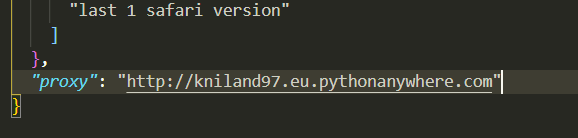
\includegraphics[width=13cm,height=5cm,keepaspectratio]{images/packagejson}
\end{center}

What this does is when a user makes a request to register for an account or log into their account, the application will send the request to the link shown above (which is essentially the Flask server as seen in the last section). The request will then be handled and processed, with the appropriate action being carried out.

\newpage
\subsubsection{Advantages}
There are a number of advantages to using PythonAnywhere:

\begin{itemize}
    \item \textbf{Always running} - Even on a free tier account, PythonAnywhere
    never sleeps (compared to something like Heroku). This means real time 
    services are viable with PythonAnywhere. This proved to be very beneficial for this application since the Flask server (which is needed to allow users to register and login to an account) can always be available and requests can be made to it any time.
    \item \textbf{Easy Setup} - It does not take long to have Python-backed website up and running. In the case of the Flask server for this application, the file simply needed to be uploaded, the appropriate libraries downloaded, and the flask file itself imported into the WSGI file (which would then 'deploy' it and allow requests to be made to it).
    \item \textbf{Free} - PythonAnywhere is free to use. On a free tier account,
    web applications stay running 24/7 for 3 months. After 3 months, it will
    shut down. However, one needs only to start it up again.
\end{itemize}

\subsubsection{Disadvantages}
There are a few disadvantages to using PythonAnywhere:

\begin{itemize}
    \item \textbf{Python-only on the server side} - You are free to use
    JavaScript in your web pages and so on, but you can't use Rails or Node on 
    the server side of things.
    \item \textbf{No WebSocket Support} - A WebSocket is a computer communications protocol, providing full-duplex communication channels over a single TCP connection. PythonAnywhere currently doesn't support WebSockets.
\end{itemize}

\newpage
\subsection{MongoDB}
\par
\medskip
\begin{center}
    
\includegraphics[width=8cm,height=3.3cm,keepaspectratio]{images/mongodb}
\end{center}
MongoDB is a cross-platform document-oriented database program \cite{mongo_docs}. Classified as a
NoSQL database program, MongoDB uses JSON-like documents with schema. Some of 
the main features of MongoDB are:

\begin{itemize}
    \item Ad-hoc queries (MongoDB supports field, range query, and
    regular-expression searches)
    \item Indexing (Fields in a MongoDB document can be indexed with primary and
    secondary indices)
    \item File storage (MongoDB can be used as a file system, called GridFS,
    with load balancing and data replication features over multiple machines for
    storing files)  
\end{itemize}

For this project, MongoDB was used as the main database. It stores user details
and user sorts. To write to the database, a request is first made through the 
application. Using a proxy, these requests are delegated to a flask application.
The flask application then processes the request and will then access the 
database to perform a certain action (such as writing user details to the 
database, accessing user details, storing user sorts, etc). 

\begin{center}
    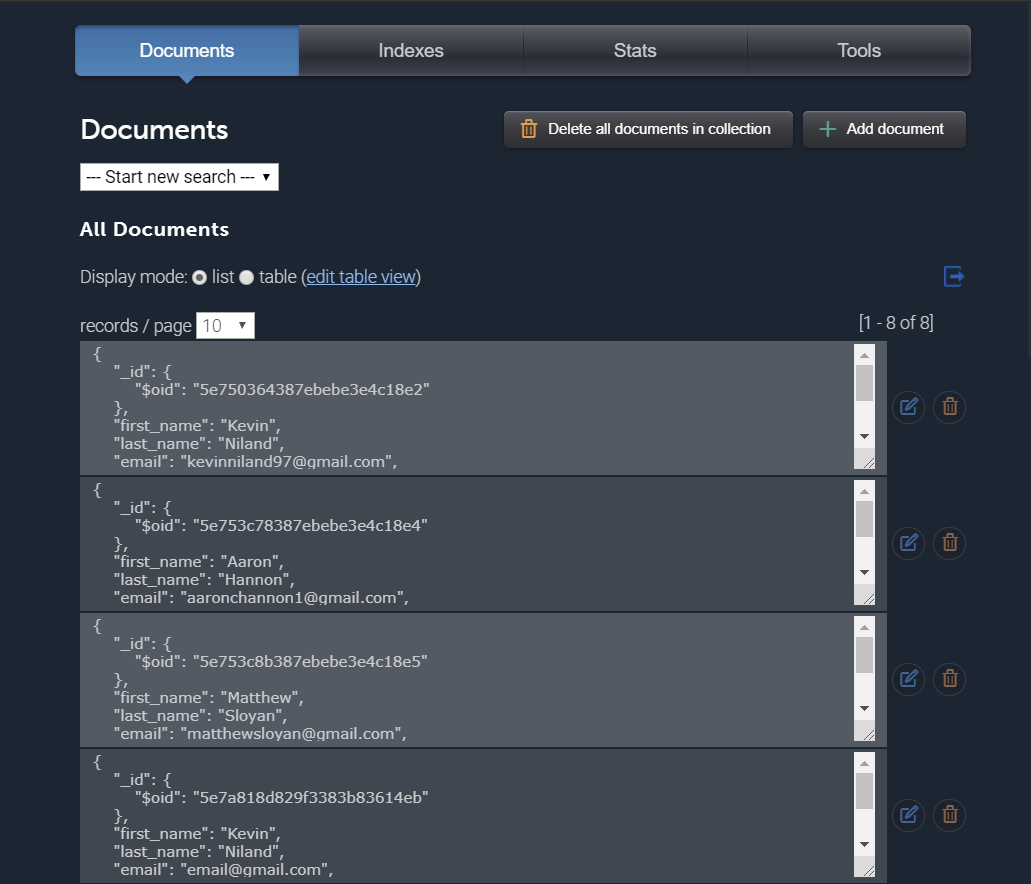
\includegraphics[width=13cm,height=7cm,keepaspectratio]{images/mlab}
\end{center}

\subsubsection{Advantages}
There are a number of advantages to using MongoDB:

\begin{itemize}
    \item \textbf{Schema-less NoSQL Database} - MongoDB is a schema-less NoSQL
    database, meaning there is no need to design the schema of the database when
    using MongoDB. The code defines the schema.
    \item \textbf{Performace} - Performance of MongoDB is much higher than
    compared to any relational database.
    \item \textbf{Internal Memory} - MongoDB uses internal memory for storage
    which enables faster access to the data.
    \item \textbf{No Joins} - MongoDB doesn't use complex joins. There is no
    relationship among data in MongoDB.
    \item \textbf{JSON} - MongoDB supports JSON. Because MongoDB uses JSON
    format to store data, it is very easy to store arrays and objects.
\end{itemize}

\subsubsection{Disadvantages}
There are a few disadvantages to using MongoDB:

\begin{itemize}
    \item \textbf{High Memory} - MongoDB uses high memory for data storage.
    \item \textbf{Document Size Limit} - MongoDB has a limit to the size of
    documents it can store.
    \item \textbf{Lack Of Transaction Support} - MongoDB does not support
    transactions.
\end{itemize}
\par
\medskip
\par
\medskip

\newpage
\subsection{Firebase}
\par
\medskip
\begin{center}
    
\includegraphics[width=8cm,height=3.3cm,keepaspectratio]{images/firebase}
\end{center}
Firebase is a mobile and web application development platform developed by Firebase, Inc \cite{firebase_docs}. With this project, Firebase was used to store the saved sorts and to host the application.

\subsubsection{Storing Sorts}
To store and upload sorts to the database, a library called React Firebase File Uploader \cite{file_uploader} was used. This allows one to upload images, videos, and other files to Firebase Storage. 

\begin{center}
    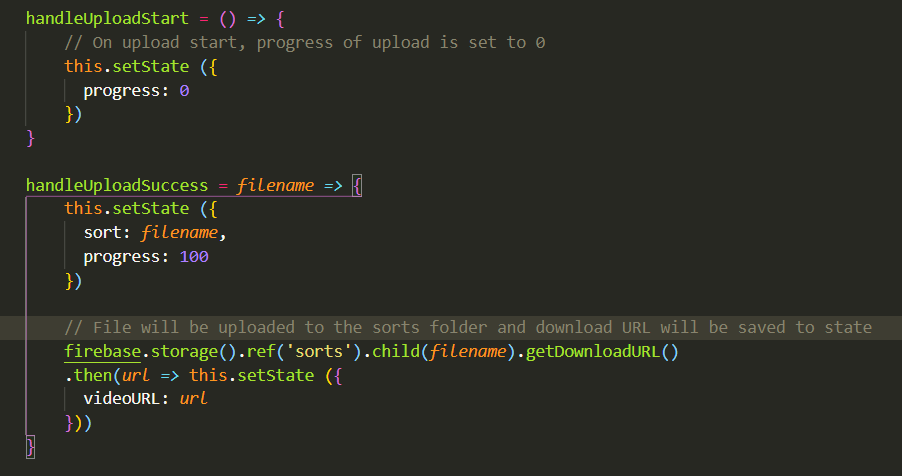
\includegraphics[width=13cm,height=9cm,keepaspectratio]{images/uploadsort}
\end{center}
As soon as the user selects a file to upload, these functions will be called and will execute accordingly. Once the file has finished uploading, it will be stored in the \lstinline{sorts} directory in Firebase Storage, from which it will then be retrieved and listed.

\newpage
\begin{center}
    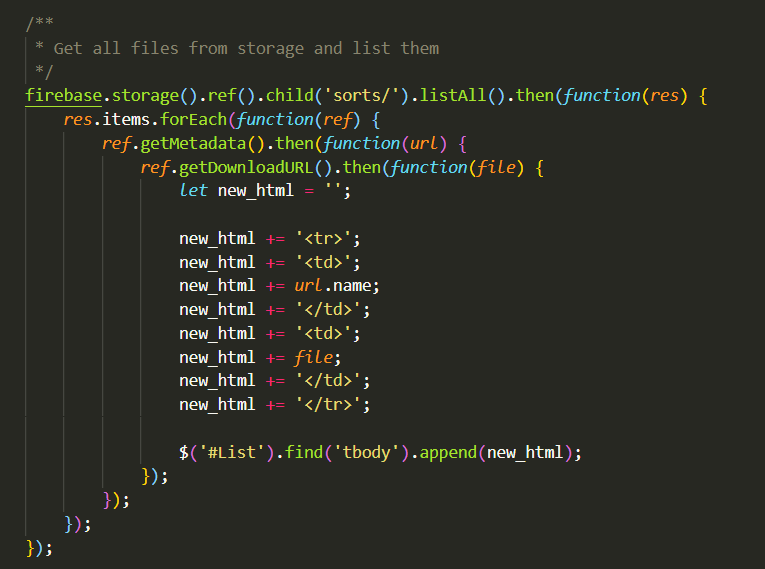
\includegraphics[width=13cm,height=9cm,keepaspectratio]{images/storesorts}
\end{center}

To retrieve and list all files from Firebase Storage, there seems to be no clear cut way to do it purely with React. To achieve this, I had to use a mix of HTML and JavaScript \cite{firebase_listing}. As can be seen above, Firebase itself has a lot of inbuilt functions to retrieve files from storage. First, all files stored in storage were retrieved. A download link for each file was then generated. To get around this, I had to use a library called React HTML Parser \cite{react_html_parser}. 

\begin{center}
    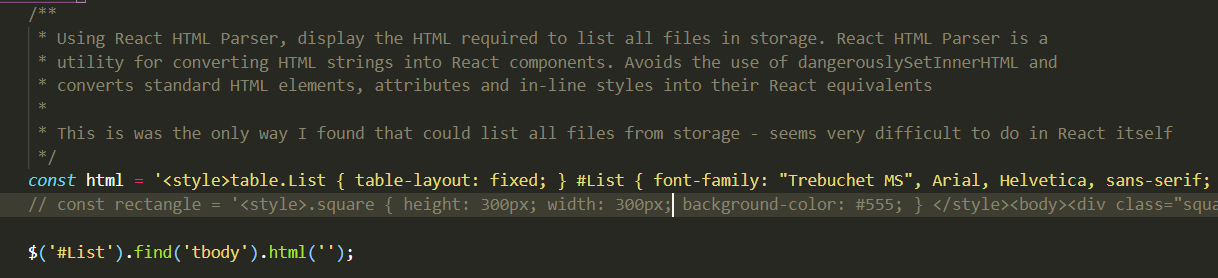
\includegraphics[width=13cm,height=9cm,keepaspectratio]{images/htmlparser}
\end{center}

This allows you define HTML code which can then be rendered using \lstinline{{ReactHtmlParser(html)}} in the \lstinline{render()} method. To style the HTML, I simply added style tags in the constant \lstinline{html}.